\documentclass[12pt]{scrartcl}

\setlength{\parindent}{0pt}
\setlength{\parskip}{.25cm}

\usepackage{graphicx}

\usepackage{xcolor}

\definecolor{darkred}{rgb}{0.5,0,0}
\definecolor{darkgreen}{rgb}{0,0.5,0}
\usepackage{hyperref}
\hypersetup{
  letterpaper,
  colorlinks,
  linkcolor=red,
  citecolor=darkgreen,
  menucolor=darkred,
  urlcolor=blue,
  pdfpagemode=none,
  pdftitle={CSCE 156 Lab Handout},
  pdfauthor={Christopher M. Bourke},
  pdfsubject={},
  pdfkeywords={}
}

\definecolor{MyDarkBlue}{rgb}{0,0.08,0.45}
\definecolor{MyDarkRed}{rgb}{0.45,0.08,0}
\definecolor{MyDarkGreen}{rgb}{0.08,0.45,0.08}

\definecolor{mintedBackground}{rgb}{0.95,0.95,0.95}
\definecolor{mintedInlineBackground}{rgb}{.90,.90,1}

%\usepackage{newfloat}
\usepackage[newfloat=true]{minted}
\setminted{mathescape,
               linenos,
               autogobble,
               frame=none,
               framesep=2mm,
               framerule=0.4pt,
               %label=foo,
               xleftmargin=2em,
               xrightmargin=0em,
               startinline=true,  %PHP only, allow it to omit the PHP Tags *** with this option, variables using dollar sign in comments are treated as latex math
               numbersep=10pt, %gap between line numbers and start of line
               style=default, %syntax highlighting style, default is "default"
               			    %gallery: http://help.farbox.com/pygments.html
			    	    %list available: pygmentize -L styles
               bgcolor=mintedBackground} %prevents breaking across pages
               
\setmintedinline{bgcolor={mintedBackground}}
\setminted[text]{bgcolor={mintedBackground},linenos=false,autogobble,xleftmargin=1em}
%\setminted[php]{bgcolor=mintedBackgroundPHP} %startinline=True}
\SetupFloatingEnvironment{listing}{name=Code Sample}
\SetupFloatingEnvironment{listing}{listname=List of Code Samples}

\title{CSCE 156 -- Computer Science II}
\subtitle{Lab 12.0 - Recursion}
\author{~}
\date{~}

\begin{document}

\maketitle

\section*{Prior to Lab}

\begin{enumerate}
  \item Review this laboratory handout prior to lab.
  \item Review the lecture notes on recursion.
\end{enumerate}

\section*{Lab Objectives \& Topics}
Following the lab, you should be able to:
\begin{itemize}
  \item Be familiar with recursive methods in the Java programming 
    language
  \item Be able to evaluate and empirically analyze recursive methods
\end{itemize}


\section*{Peer Programming Pair-Up}

To encourage collaboration and a team environment, labs will be
structured in a \emph{pair programming} setup.  At the start of
each lab, you will be randomly paired up with another student 
(conflicts such as absences will be dealt with by the lab instructor).
One of you will be designated the \emph{driver} and the other
the \emph{navigator}.  

The navigator will be responsible for reading the instructions and
telling the driver what to do next.  The driver will be in charge of the
keyboard and workstation.  Both driver and navigator are responsible
for suggesting fixes and solutions together.  Neither the navigator
nor the driver is ``in charge.''  Beyond your immediate pairing, you
are encouraged to help and interact and with other pairs in the lab.

Each week you should alternate: if you were a driver last week, 
be a navigator next, etc.  Resolve any issues (you were both drivers
last week) within your pair.  Ask the lab instructor to resolve issues
only when you cannot come to a consensus.  

Because of the peer programming setup of labs, it is absolutely 
essential that you complete any pre-lab activities and familiarize
yourself with the handouts prior to coming to lab.  Failure to do
so will negatively impact your ability to collaborate and work with 
others which may mean that you will not be able to complete the
lab.  


\section*{Recursion}

Recursion is a programming approach common to a ``divide and conquer'' 
algorithm strategy where a problem is deconstructed into smaller 
sub-problems until a ``base case'' is reached and the problem is 
solved directly.  This lab will get you familiar with recursive 
algorithms by taking you through several exercises to design and 
analyze recursive algorithms.  

Clone the starter code for this lab from GitHub using the following
url: \url{https://github.com/cbourke/CSCE156-Lab12}.

\section*{Analyzing the Fibonacci Sequence}

Recall that the Fibonacci sequence is a recursively defined sequence 
such that each term is the sum of the sequence?s two previous terms.  
That is, the sequence
  $$1, 1, 2, 3, 5, 8, 13, 21, 34, 55, \ldots$$
A recursive method to compute the Fibonacci sequence has been provided 
for you (see \mintinline{java}{unl.cse.recursion.Fibonacci}).  The 
\mintinline{java}{main()} method of this class also provides code to 
compute the execution time of the recursive method.  Run the program 
for several input instances.  

This recursive method is highly inefficient: the method is called 
many times on the same input.  Your task will be to directly observe 
this by adding code to count the exact number of times the method is 
called for each input $n$.

To do this, declare a private integer array and increment entries on 
each call to the recursive method depending on the input n.  You may 
assume that an array no larger than 50 will be needed.

\section*{Palindromes}

A \emph{palindrome} is a string of characters that is the same 
string when reversed.  Examples of palindromes: kayak, abba, 
noon.  An empty string and any string of length one is a palindrome 
by definition.  

Your task will be to design and implement a recursive algorithm to 
determine if a given string is a palindrome or not.  Implement the 
method in the class \mintinline{java}{unl.cse.recursion.Palindrome}.
You may find that Java's \mintinline{java}{String} class has several 
useful methods such as \mintinline{java}{charAt(int)} and 
\mintinline{java}{substring(int, int)}.

\section*{Sierpinski Triangle}

A fractal is a geometric object that is self-similar.  That is, 
if you zoom in on the object, it retains the same appearance or 
structure.  One such fractal is the Sierpinski Triangle which is 
formed by drawing a triangle and removing an internal triangle 
drawn by connecting the midpoints of the outer triangle's sides.  
This process is repeated recursively ad infinitum.  This process is illustrated for the first four iterations in Figure \ref{figure:sierpinski}.

\begin{figure}
\centering
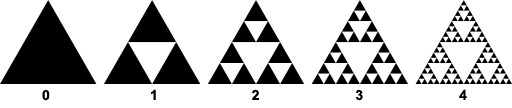
\includegraphics[scale=0.75]{sierpinski}
\caption{Sierpinski Triangle, 4 iterations}
\label{figure:sierpinski}
\end{figure}
 
A Java applet has been provided to you (
\mintinline{java}{unl.cse.recursion.SierpinskiTriangle}) that 
recursively draws the Sierpinski Triangle for a specified number 
of recursive iterations.  Since this is an applet, you can run it 
without having a \mintinline{java}{main()} method.  The depth of 
the recursion is specified in the \mintinline{java}{paint()} 
method.  It will be your task to modify this program to count 
the total number of triangles that a recursion of depth n will 
ultimately render.

\section*{Pell Numbers}

Another recursively defined sequence similar to the Fibonacci 
sequence are the Pell Numbers, defined as follows.

$$P_n = \left\{
\begin{array}{ll}
0 & \textrm{if } n=0 \\
1 & \textrm{if } n=1 \\
2P_{n-1}+P_{n-2} & \textrm{otherwise}
\end{array}
\right.$$
 
A program has been provided (\mintinline{java}{PellNumbers}) that 
computes the n-th Pell Number using a recursive function.  The method 
has been defined using Java's \mintinline{java}{BigInteger} class, 
a class that supports arbitrary precision integers.  If we were to 
use this implementation to compute the 1000-th Pell Number, the 
computation would take not just centuries, but billions and billions 
of years!!

One alternative to such inefficient recursion is to use \emph{memoization}.  
Memoization typically involves defining and filling a tableau of 
incremental values whose values are combined to compute subsequent 
values in the table.  

For this exercise, we will instead use a Java \mintinline{java}{HashMap} 
to store values.  A \emph{map} is a data structure that allows you 
to define and retrieve key-value pairs.  For this exercise, define 
a (static) \mintinline{java}{HashMap} that maps \mintinline{java}{Integer} types to \mintinline{java}{BigInteger} types ($n$ to $P_n$) and use 
it in the \mintinline{java}{PellNumber} method as follows.  If
the value $P_n$ is already defined in the map, use it as a return 
value.  Otherwise, compute the value using recursion, but also place 
the result into the \mintinline{java}{HashMap} so that it will be 
available for subsequent recursive calls.

Answer the questions in your worksheet and demonstrate your working 
programs to a lab instructor.

\section*{Submission}

We have included a test suite of unit tests written in JUnit 
(\url{https://junit.org/junit5/}) a popular unit testing framework for
Java.  Even though the test driver (in the \mintinline{text}{src/test}
source folder) has no main method, you can still run it in Eclipse and
get a report on how many of the tests passed, failed or resulted in 
an unexpected exception.  Be sure all of the unit tests pass before
submitting your source files through webhandin.  You can rerun this
test suite in the webgrader to ensure everything works.  

\section*{Advanced Activity (Optional)}

Bonus Activity 1: The Fibonacci method in Case Study 1 returns a 
primitive Java \mintinline{java}{int} value which has a maximum 
possible value of 2,147,483,647.  Find the maximum value n such 
that this method returns an accurate value (the value n such that 
calling \mintinline{java}{Fibonacci(n+1)} results in overflow).  
Hint: you probably cannot use the recursive version provided 
(why?).  Write an alternative method to compute the Fibonacci 
sequence that returns a Java \mintinline{java}{BigInteger} (an 
arbitrary-precision number class).  Also use memoization to 
eliminate repeated recursive calls.

\end{document}
